\section{HEC-RAS Confluence (Junctions)}
%%%%%%%%%%%%%%%%%%%%%%%%%%%
what is a junction?
how are they conceptualized?
options for simulation 

\subsection{Conceptualization}

\subsubsection{Tributary does not directly contribute momentum to main branch }

\subsubsection{Tribuitary directly contributes momentum to main branch}


\clearpage
\subsection{Examples}
\subsubsection{Example 1. -- using HEC-RAS Steady}

Figure  \ref{fig:confluence} is a sketch of a channel and tributary system with a road (bridge) crossing the main channel.  The cross sections are surveyed and the sections are included in Figure \ref{fig:cross-sections-table}

\begin{figure}[h!] %  figure placement: here, top, bottom, or page
   \centering
   \includegraphics[width=4.5in]{confluence.png} 
   \caption{Plan view/schematic for example}
   \label{fig:confluence}
\end{figure}

Cross section 1 is the most downstream section; sections 10 and 14 are upstream sections.  
Roughness coefficients for the left-over-bank, channel, and right-over-bank are estimated as 0.10, 0.05, and 0.08 for the main channel portion of the system and 0.08, 0.05, and 0.08 for the tributary portion of the system.
\clearpage
Figure \ref{fig:cross-sections-table} is a screen capture of a data table that contains the location of the cross sections relative to the diagram (Section 1 is located at distance 0 from the outlet, Section 10 is located 1760 feet upstream of the outlet, etc.).  
The numbers to the right of each section title in the table are the distances upstream from section 1 and should be used as the section names in HEC-RAS.   
\begin{figure}[h!] %  figure placement: here, top, bottom, or page
   \centering
   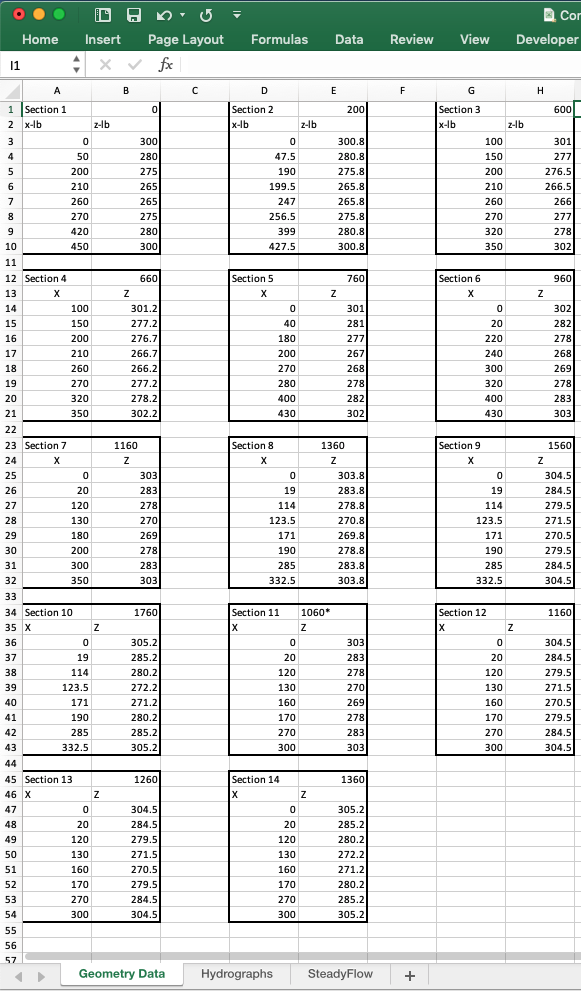
\includegraphics[height=5in]{cross-sections-table.png} 
   \caption{Tabular cross sections }
   \label{fig:cross-sections-table}
\end{figure}
Section 11 connects to the main channel between Section 6 and 7, and that is the meaning of the ``*'' symbol in the table.
The angle that the tributary forms with the main channel is about 60-degrees.
X-LB and Z-LB are distance and elevation relative to the left bank of each section. %--- Figure 2 is a plot of Section 3 for reference.

The road is cut into the surrounding grade so that the low chord of the bridge at the main channel is at elevation 290, and the roadway surface is at elevation 295 feet.  
\clearpage
Figure \ref{fig:steady-flow-conditions} is a table of steady flow conditions to consider. 

\begin{figure}[h!] %  figure placement: here, top, bottom, or page
   \centering
   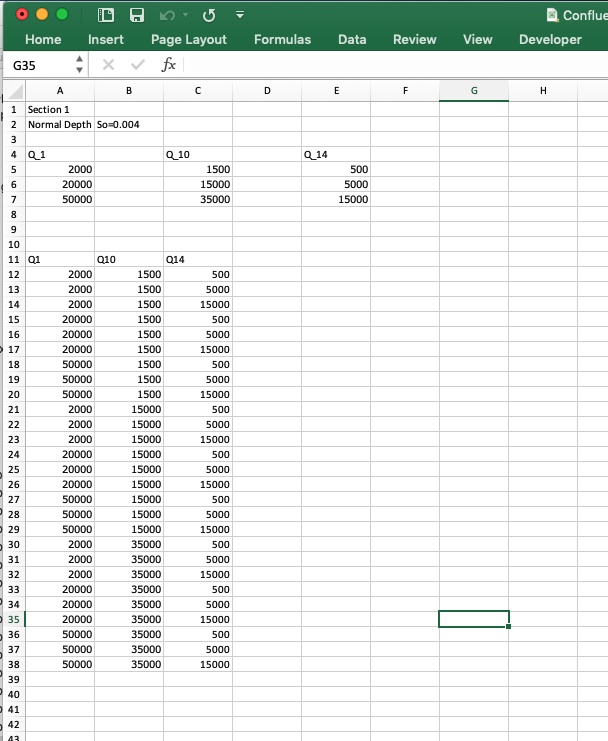
\includegraphics[height=5in]{steady-flow-conditions.png} 
   \caption{Steady flow conditions - various combinations}
   \label{fig:steady-flow-conditions}
\end{figure}
Determine if the current bridge low chord can accommodate the different flows. 
If flow cannot clear the low chord, treat the bridge as a large culvert and determine if the roadway surface is still passable (not flooded).

Repeat the analysis assuming the bridge abutments extend 100 feet into the left and right over-bank.
\clearpage
Figure \ref{fig:hydrographs-table} is a table of transient flow conditions to consider. 
\begin{figure}[h!] %  figure placement: here, top, bottom, or page
   \centering
   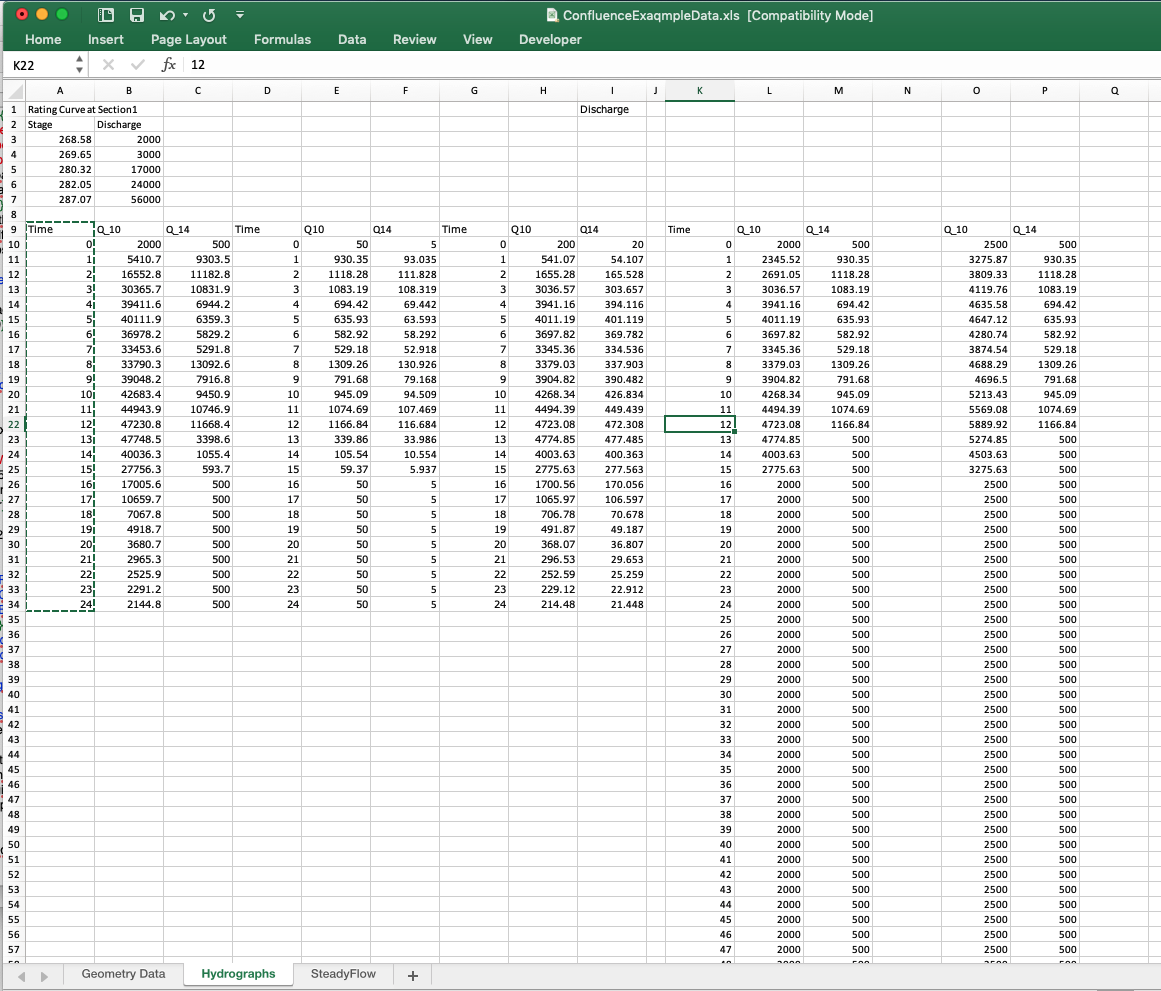
\includegraphics[height=5in]{hydrographs-table.png} 
   \caption{Transient flow conditions }
   \label{fig:hydrographs-table}
\end{figure}
\newline
Determine if the current bridge low chord can accommodate the different flows.  


If flow cannot clear the low chord, treat the bridge as a large culvert and determine if the roadway surface is still passable (not flooded).

Repeat the analysis assuming the bridge abutments extend 100 feet into the left and right over-bank.






\subsection{Appendix}
